\documentclass{beamer}
\usefonttheme[onlymath]{serif}
\usepackage{ctex, hyperref}
\usepackage[T1]{fontenc}

% other packages
\usepackage{latexsym,amsmath,xcolor,multicol,booktabs,calligra}
\usepackage{graphicx,pstricks,listings,stackengine}
\usepackage{multirow}

\author{匿名}
\title{基于可信执行环境的高性能加密重复数据删除研究}
\subtitle{硕士学位论文答辩}
\institute{电子科技大学计算机科学与工程学院(网络空间安全学院)}
\date{2022年5月13日}
\usepackage{UESTC}

% defs
\def\cmd#1{\texttt{\color{red}\footnotesize $\backslash$#1}}
\def\env#1{\texttt{\color{blue}\footnotesize #1}}
\definecolor{deepblue}{rgb}{0,0,0.5}
\definecolor{deepred}{rgb}{0.6,0,0}
\definecolor{deepgreen}{rgb}{0,0.5,0}
\definecolor{halfgray}{gray}{0.55}

\lstset{
    basicstyle=\ttfamily\small,
    keywordstyle=\bfseries\color{deepblue},
    emphstyle=\ttfamily\color{deepred},    % Custom highlighting style
    stringstyle=\color{deepgreen},
    numbers=left,
    numberstyle=\small\color{halfgray},
    rulesepcolor=\color{red!20!green!20!blue!20},
    frame=shadowbox,
}

\newcommand{\sysnameS}{TEEDedup }
\newcommand{\sysnameF}{FeatureSpy }
\newcommand{\prototype}{TEEDedup+ }

\begin{document}

\kaishu
\begin{frame}
    \titlepage
\end{frame}

% \begin{frame}
%     \tableofcontents[sectionstyle=show,subsectionstyle=show/shaded/hide,subsubsectionstyle=show/shaded/hide]
% \end{frame}


\section{研究背景}

% \begin{frame}{外包数据存储}
%     \begin{itemize}[<+-| alert@+>] % 当然,除了alert,手动在里面插 \pause 也行
%         \item Outsourcing data management to cloud is common in practice
%         \item 22% business data are stored in the cloud[*]
%         \item  Outsourcing storage should fulfill security and storage efficiency
%         \item  Security: protect outsourced data against unauthorized access
%         \item  Storage efficiency: reduce storage footprints
%     \end{itemize}
% \end{frame}

\begin{frame}{外包数据存储}
    \begin{itemize}
        \item 外包数据存储管理的数据规模快速增长
              \begin{itemize}
                  \item 根据IDC发布于2020年的预测,2025年时单年新创建数据量将超过175.8\,ZB,且其中超过70\%的数据将集中存储于云端
              \end{itemize}
    \end{itemize}
    \vspace{-1em}
    \begin{figure}[!htb]
        \centering
        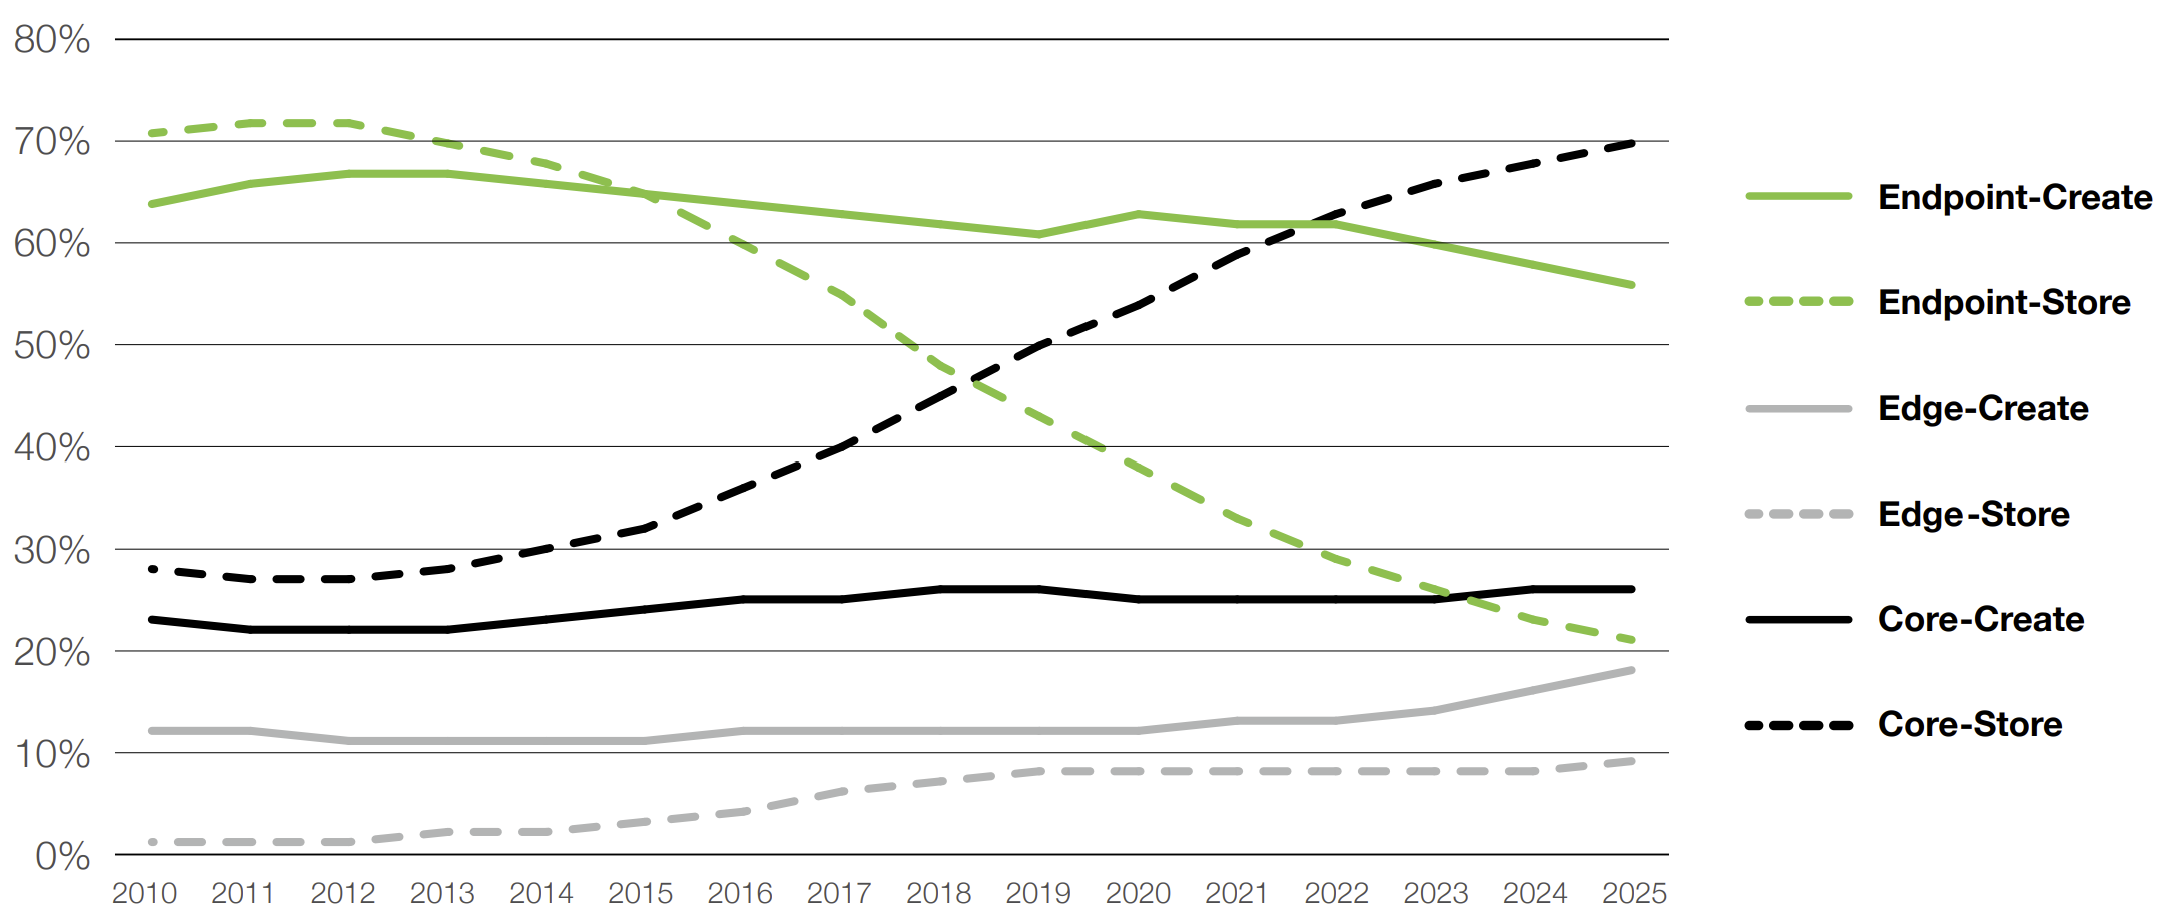
\includegraphics[width=0.8\linewidth]{./pic/dataStore.png}
        \vspace{-5pt}
        \caption{数据产生与存储关系的统计与预测}
        \label{fig:dataCreateAndStore}
    \end{figure}
    \vspace{-1.5em}
    \begin{itemize}
        \item  外包数据存储需同时满足安全性和存储经济性需求
              \begin{itemize}
                  \item 安全性:保护外包数据免受未授权访问
                  \item 存储经济性:尽可能减少存储设备需求
              \end{itemize}
    \end{itemize}
\end{frame}

\begin{frame}{重复数据删除}
    \begin{figure}[!htb]
        \small
        \centering
        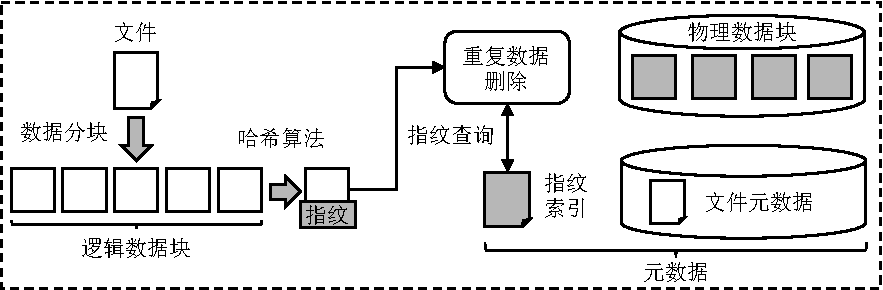
\includegraphics[width=\linewidth]{../pic/background/chunk-based-dedup-arch.pdf}
        \caption{基于数据块的重复数据删除的工作流程概览}
        \label{fig:chunk-based-dedup-flow}
    \end{figure}
    \vspace{-1em}
    \begin{itemize}
        \item 重复数据删除是一种粗粒度的数据压缩技术
              \begin{itemize}
                  \item 作用单位为数据块(可变大小或固定大小)
              \end{itemize}
        \item  其进保存具有相同内容的数据块的一个副本,并将其他数据块通过索引指向该副本
    \end{itemize}
\end{frame}

\begin{frame}{加密重复数据删除}
    \begin{figure}[!htb]
        \small
        \centering
        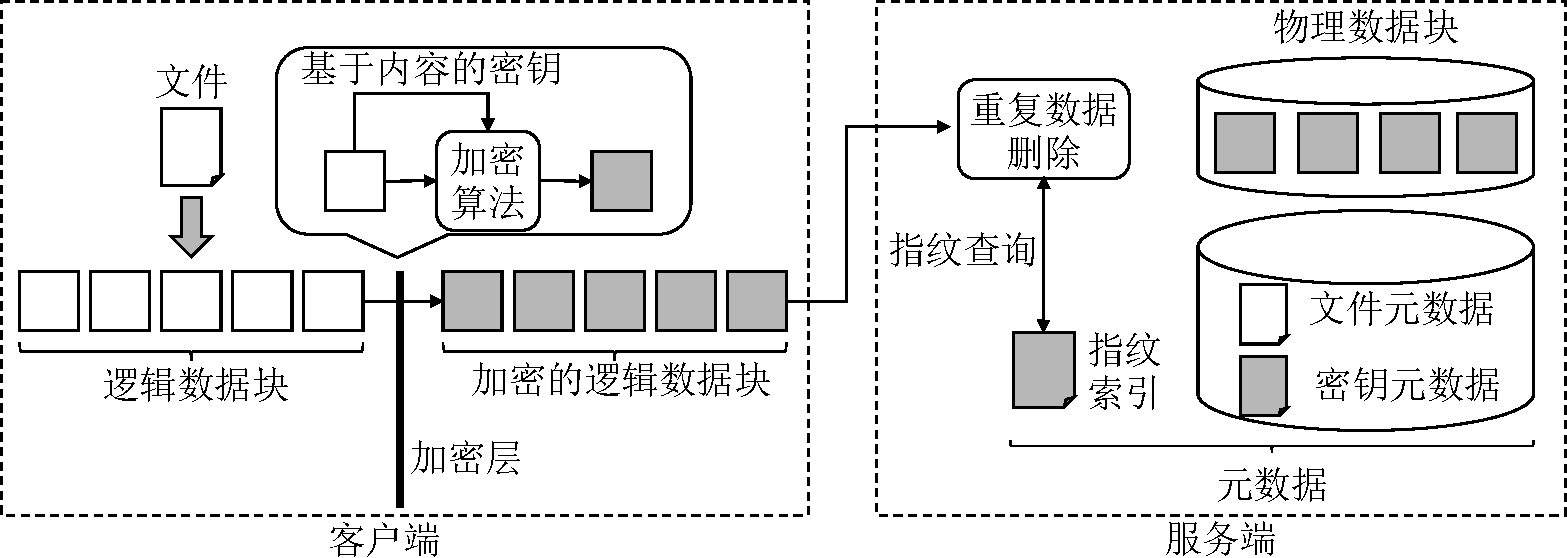
\includegraphics[width=\textwidth]{../pic/background/chunk-based-enc-dedup-arch.pdf}
        \caption{基于数据块的加密重复数据删除的工作流程概览}
        \label{fig:chunk-based-enc-dedup-flow}
    \end{figure}
    \vspace{-1em}
    \begin{itemize}
        \item 加密重复数据删除基于密文数据块执行重复数据删除
              \begin{itemize}
                  \item 传统加密方案无法兼容跨用户的重复数据删除
                  \item 消息锁加密基于明文数据块导出加密密钥(例如数据块哈希)
              \end{itemize}
    \end{itemize}
\end{frame}

\begin{frame}{加密重复数据删除的安全性保障}
    \begin{figure}[!htb]
        \small
        \centering
        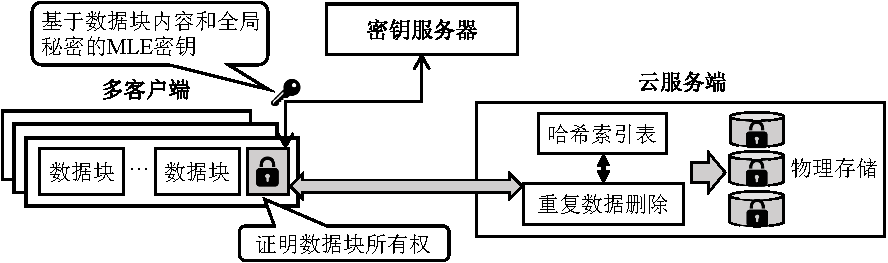
\includegraphics[width=\textwidth]{../pic/background/Cloud-encrypted-deduplication-logic.pdf}
        \caption{面向云环境的加密重复数据删除系统框架}
        \label{fig:Cloud-based-encrypted-deduplication-storage-logic}
    \end{figure}
    \vspace{-1em}
    \begin{itemize}
        \item 依赖基于盲签名的服务器辅助密钥生成抵御离线暴力破解攻击
        \item 依赖数据所有权证明保护源端重复数据删除(即仅传输非重复数据块)
              \begin{itemize}
                  \item 目标端重复数据删除需传输所有数据块,产生高额网络资源开销
              \end{itemize}
    \end{itemize}
\end{frame}

\begin{frame}{性能瓶颈问题}
    \begin{table}[!htb]
        \small
        \centering
        \caption{基础原型每个步骤处理1MiB数据的时间开销:括号内为可供备选的服务器辅助密钥生成方案和所有权证明方案,以及相应处理时间}
        \label{tab:intro-bottleneck}
        \begin{tabular}{@{}ccc@{}}
            \toprule
                                        & 处理阶段/可选方案            & 处理时间(ms/MiB) \\ \midrule
                                        & 数据分块                     & 3.8              \\
            服务器辅助密钥生成          & RSA(BLS)盲签名方案 & 40.7(488.3)      \\
            \multirow{3}{*}{所有权证明} & 数据加密                     & 2.5              \\
                                        & Merkel树(通用哈希)方案     & 27.0(7.2)        \\
                                        & 重复数据删除                 & 1.7              \\ \bottomrule
        \end{tabular}
    \end{table}
    \begin{itemize}
        \item 盲签名(OPRF)算法成为加密重复数据删除的系统性能瓶颈
        \item 基于Merkel树的所有权证明方案安全但计算开销极大
        \item 基于通用哈希的方案以降低安全性为代价且仍为性能瓶颈之一
    \end{itemize}
\end{frame}

\begin{frame}{安全性问题—推测内容攻击}
    \begin{itemize}
        \item 通过枚举可能的目标内容进行重复数据删除查询,基于重复数据删除结果判断攻击成功与否
    \end{itemize}
    \begin{figure}[!htb]
        \small
        \centering
        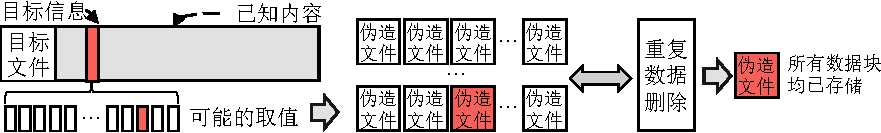
\includegraphics[width=\textwidth]{./pic/LRI.pdf}
        \caption{推测内容攻击模式}
        \label{fig:LRI-mode}
    \end{figure}
    \vspace{-1em}
    \begin{itemize}
        \item 现有防御机制存在高额网络资源开销或安全性不足等问题
        \begin{itemize}
            \item 目标端重复数据删除(Target-based deduplication)
            \item 随机阈值重复数据删除(Randomized-threshold deduplication)
            \item 两阶段重复数据删除(Two-stage deduplication)
            \item 随机冗余数据块传输方案(Randomized Redundant Chunk Scheme)
    \end{itemize}
    \end{itemize}
\end{frame}

\begin{frame}{可信执行环境}
    \begin{itemize}
        \item 可信执行环境(TEE)是一种在计算平台上由软硬件协同构建的安全区域,可确保其中的程序按照预期执行,保证程序初始状态和运行时的机密性、完整性
        \begin{itemize}
            \item \textbf{隔离性}:
                  TEE将其中的目标程序、数据等与外部环境隔离,使得TEE外软硬件均无法获得其内部的机密信息。
            \item \textbf{软硬协同性}:
                  TEE产品包含物理隔离的专用硬件或运行权限以及相应的软件SDK。
            \item \textbf{富表达性}:
                  与传统安全芯片或纯软件的密码学隐私保护机制相比,TEE支持更丰富的上层应用。
        \end{itemize}
        \item  主流可信执行环境
              %   \vspace{-1em}
              \begin{itemize}
                  \item  Intel SGX:拥有隔离、密封、远程认证能力,已被广泛运用于安全虚拟机等场景
                  \item  ARM TrustZone:通过CPU状态切换实现隔离,并支持专用安全外设,已被广泛运用于移动设备生物识别、安全存储等场景
              \end{itemize}
    \end{itemize}
\end{frame}

\section{研究内容}

\begin{frame}{研究内容概述}
    \begin{itemize}
        \item 针对现有面向云环境的加密重复数据删除存在密钥生成效率低、所有权证明计算复杂、易于遭受推测内容攻击等不足,提出:
              \begin{itemize}
                \item 基于TEE的轻量级密钥生成技术,相较基于RSA盲签名的方案实现{\color{red}131倍}性能提升
                \item 基于TEE的高效所有权证明技术,相较基于Merkel树的方案实现{\color{red}8.2倍}性能提升
                \item 基于TEE的扩展所有权证明技术,在测试数据集中实现{\color{red}99\%}以上的检测成功率
              \end{itemize}
    \end{itemize}
    \begin{itemize}
        \item 设计并分别实现基于Intel SGX和ARM TrustZone的\prototype 原型系统:
              \begin{itemize}
                \item 相较于基于密码学方案的DupLESS实现{\color{red}8.1$\sim$9.6倍}的性能提升
                \item 相较于不采用任何安全措施的明文重复数据删除系统仅产生{\color{red}17.5\%}的额外开销
              \end{itemize}
    \end{itemize}
\end{frame}

\subsection{\sysnameS: 基于TEE加速加密重复数据删除}

\begin{frame}{\sysnameS: 基于TEE加速加密重复数据删除}
    \begin{figure}[!htb]
        \centering
        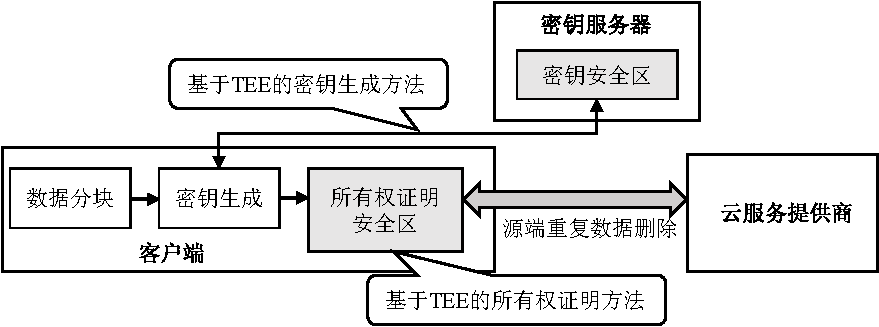
\includegraphics[width=\linewidth]{../pic/sgxdedup/sgxdedup-arch.pdf}
        \caption{\sysnameS 系统框架,在密钥服务器和每个客户端中分别部署了密钥安全区和所有权证明安全区}
        \label{fig:sgxdedup-overview}
    \end{figure}
    \vspace{-1em}
    \begin{itemize}
        \item  核心思想:使用TEE取代加密重复数据删除中计算开销高昂的基于密码学算法
    \end{itemize}
\end{frame}

\begin{frame}{基于TEE的数据所有权证明}
    \begin{figure}[!htb]
        \centering
        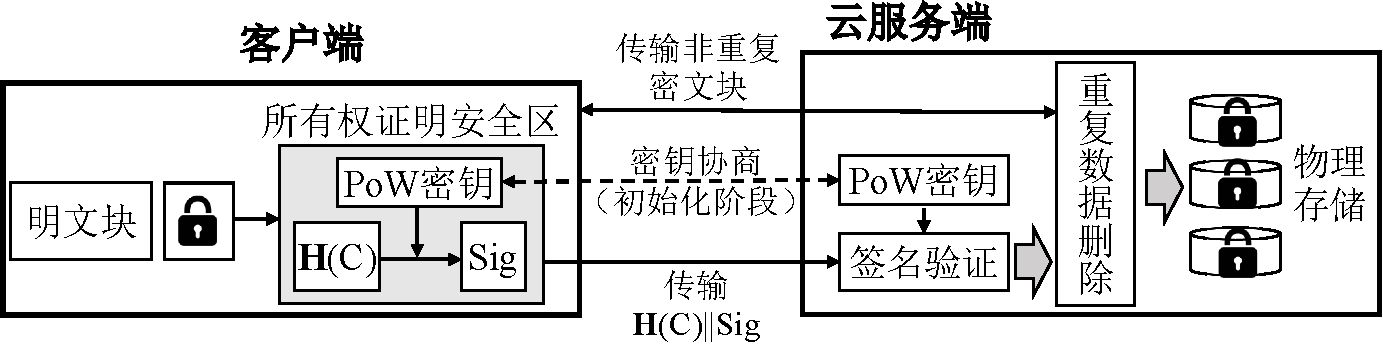
\includegraphics[width=\textwidth]{../pic/sgxdedup/pow.pdf}
        \caption{\sysnameS 所有权证明安全区}
        \label{fig:sgxdedup-overview-pow}
    \end{figure}
    \vspace{-1em}
    \begin{itemize}
        \item  基于安全区与云服务端共享的PoW密钥对数据块进行指纹计算并签名,取代昂贵的Merkel树构建和验证
    \end{itemize}
\end{frame}

\begin{frame}{基于TEE的推测性加密}
    \begin{figure}[!htb]
        \centering
        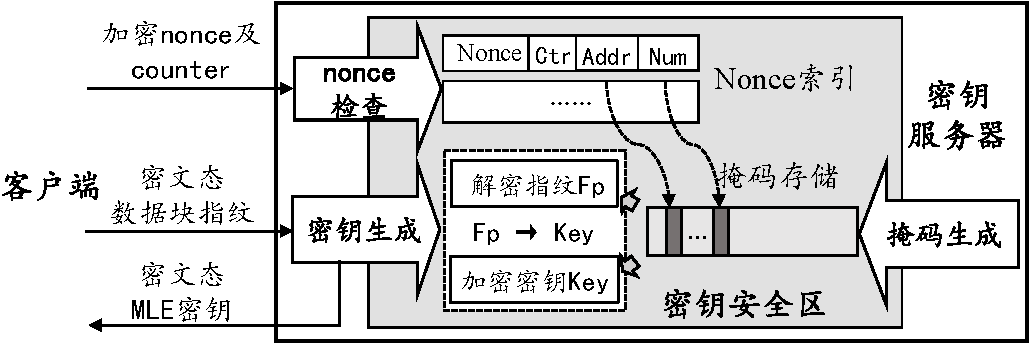
\includegraphics[width=\textwidth]{../pic/sgxdedup/key-enclave-arch.pdf}
        \caption{基于TEE的推测性加密概述}
        \label{fig:sgxdedup-SpecEnc}
      \end{figure}
      \vspace{-1em}
      \begin{itemize}
        \item  基于密钥安全区和客户端共享的会话密钥保护密钥生成过程
        \item 基于AES CTR模式进行会话内容加解密,密钥安全区离线生成CTR模式所需的加解密掩码以提升在线服务效率
    \end{itemize}
\end{frame}

\begin{frame}{基于TEE的自更新会话密钥管理}
    \begin{figure}[!htb]
        \centering
        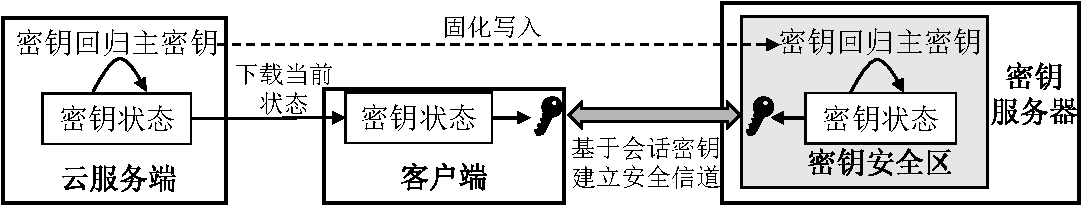
\includegraphics[width=\textwidth]{../pic/sgxdedup/keyRegression.pdf}
        \caption{自更新的会话密钥管理}
        \label{fig:sgxdedup-keymanage}
      \end{figure}
      \vspace{-1em}
      \begin{itemize}
        \item 云服务端和密钥安全区可以根据其会话密钥状态导出新的会话密钥,而客户端只能从云服务端下载当前密钥状态,并产生最新的会话密钥
        \item 仅有通过认证的客户端可获取最新的会话密钥状态,实现云服务端对云存储服务订阅的动态管理
    \end{itemize}
\end{frame}

\subsection{\sysnameF: 基于TEE在线检测推测内容攻击}

\begin{frame}{\sysnameF: 基于TEE在线检测推测内容攻击}
    \begin{figure}[!htb]
        \centering
        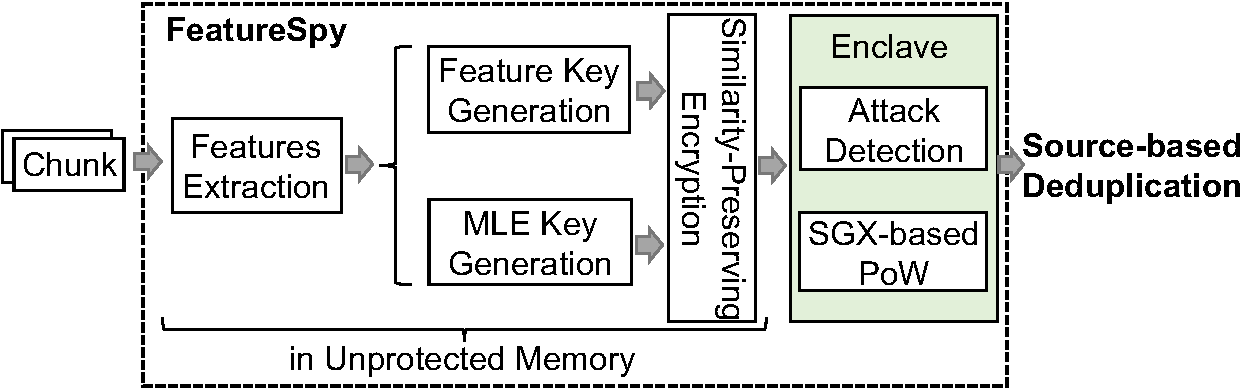
\includegraphics[width=\textwidth]{../pic/featurespy/architecture.pdf}
        \caption{基于密文的攻击检测方案工作流程。\sysnameF 将攻击检测程序与安全区中的所有权证明(\sysnameS )结合起来,以恶意客户端防止绕过检测}
        \label{fig:featurespy-architecture-secure}
    \end{figure}
    \vspace{-1em}
    \begin{itemize}
        \item 检测原理:执行推测内容攻击的客户端需枚举伪造文件,产生大量相似数据块
        \item 核心思想:在安全区中对采用相似性保留加密的数据块特征进行统计,以判断攻击是否发生
    \end{itemize}
\end{frame}

\begin{frame}{数据块特征提取}
    \begin{itemize}
        \item Outsourcing data management to cloud is common in practice
              \begin{itemize}
                  \item 22\% business data are stored in the cloud[*]
              \end{itemize}
        \item  Outsourcing storage should fulfill security and storage efficiency
              %   \vspace{-1em}
              \begin{itemize}
                  \item  Security: protect outsourced data against unauthorized access
                  \item  Storage efficiency: reduce storage footprints
              \end{itemize}
    \end{itemize}
\end{frame}

\begin{frame}{相似性保留加密}
    \begin{itemize}
        \item Outsourcing data management to cloud is common in practice
              \begin{itemize}
                  \item 22\% business data are stored in the cloud[*]
              \end{itemize}
        \item  Outsourcing storage should fulfill security and storage efficiency
              %   \vspace{-1em}
              \begin{itemize}
                  \item  Security: protect outsourced data against unauthorized access
                  \item  Storage efficiency: reduce storage footprints
              \end{itemize}
    \end{itemize}
\end{frame}

% \begin{frame}{如何使用块}
%     \begin{block}{块的名称}
%         \begin{itemize}
%             \item A
%             \item B
%         \end{itemize}
%     \end{block}
% \end{frame}

% \begin{frame}{如何使用定义、定理、引理、证明}

%     \kaishu
%     \begin{define}[定义名称]
%         定义内容
%     \end{define}

%     \begin{lem}[引理名称]
%         引理内容
%     \end{lem}

%     \begin{thm}[定理名称]
%         定理内容(这里的定义、引理、定理分章节自动标号)
%     \end{thm}

%     \begin{proof}
%         证明内容
%     \end{proof}
% \end{frame}

\section{原型系统实现}

\begin{frame}{原型系统实现}
    \begin{textbox}{基于Intel SGX}
        \begin{itemize}
            \item \prototype 及其底层\sysnameS 基于Intel SGX SDK 2.15以及OpenSSL、LevelDB等开发,包含16.5K行C++代码
            \item 开源链接:\href{https://github.com/tinoryj/masterGraduation/artifactsSGX}{https://github.com/tinoryj/masterGraduation/artifactsSGX}
        \end{itemize}
    \end{textbox}

    \begin{textbox}{基于ARM TrustZone}
        \begin{itemize}
            \item \prototype 及其底层\sysnameS 基于OP-TEE 3.16以及OpenSSL、LevelDB等开发,包含13.5K行C++代码
            \item 开源链接:\href{https://github.com/tinoryj/masterGraduation/artifactsARM}{https://github.com/tinoryj/masterGraduation/artifactsARM}
        \end{itemize}
    \end{textbox}
\end{frame}

\section{实验分析}

\subsection{测试环境}

\begin{frame}{测试环境与数据集}
    \begin{textbox}{测试数据集}
        \vspace{-1em}
        \begin{table}[!htb]
            \small
            \centering
            \caption{真实世界数据集的特征}
            \label{tab:featurespy-datasets}
            \begin{tabular}{cccc}
                \toprule
                {\bf 数据集} & {\bf 快照总数} & {\bf 去重前总数据量} & {\bf 重复数据删除系数} \\
                \midrule
                FSL          & 795            & 56.2\,TiB            & 140.4                  \\
                MS           & 143            & 14.4\,TiB            & 6.0                    \\
                Linux        & 84             & 44.9\,GiB            & 1.3                    \\
                CouchDB      & 83             & 22.9\,GiB            & 1.5                    \\
                \bottomrule
            \end{tabular}
        \end{table}
    \end{textbox}

    \begin{textbox}{测试平台}
        \begin{itemize}
            \item 本地集群(LAN)。万兆局域网内多台Intel SGX设备,每台设备均采用Intel Core i7-10700 CPU,4\,TB SATA机械硬盘,32\,GB DDR4内存
            \item 云环境(Cloud)。在两个不同区域的阿里云部署了多台规格为\textit{ecs.g7t.3xlarge}的虚拟机(VM)来分别运行云服务端、密钥服务器和多个客户端。
        \end{itemize}
    \end{textbox}
\end{frame}

\subsection{\sysnameS 原型系统}

\begin{frame}{\sysnameS 原型系统实验结果概览}
    \begin{table}[!htb]
        \small
        \centering
        \caption{\sysnameS 原型系统主要实验结果汇总}
        \label{tab:sgxdedup-summary}
        \begin{tabular}{cccc}
            \toprule
            \multicolumn{2}{c}{\bf 对比对象}                                   & {\bf 基础方案/系统}                    & {\bf 优势}                                   \\
            \midrule
            \multirow{8}{*}{\bf 性能提升}                                      & \multirow{4}{*}{\shortstack{密钥生成}} & OPRF-BLS           & 1,583$\times\;\uparrow$ \\
                                                                               &                                        & OPRF-RSA           & 131.9$\times\;\uparrow$ \\
                                                                               &                                        & MinHash encryption & 9.4$\times\;\uparrow$   \\
                                                                               &                                        & TED                & 3.7$\times\;\uparrow$   \\
            \cline{2-4}
                                                                               & \multirow{2}{*}{所有权证明}            & PoW-MT             & 8.2$\times\;\uparrow$   \\
                                                                               &                                        & PoW-UH             & 2.2$\times\;\uparrow$   \\
            \cline{2-4}
                                                                               & \multirow{2}{*}{\shortstack{原型系统}} & DupLESS            & 8.1$\times\;\uparrow$   \\
                                                                               &                                        & PlainDedup         & 17.5\% $\downarrow$     \\
            \hline
            \multicolumn{2}{c}{\multirow{2}{*}{\shortstack{\bf 网络资源节省}}} & Two-stage dedup                        & 35.3\% $\uparrow$                            \\
            \multicolumn{2}{c}{}                                               & Randomized-threshold dedup             & 91.4\% $\uparrow$                            \\
            \bottomrule
        \end{tabular}
    \end{table}
\end{frame}

\begin{frame}{密钥生成效率}
    \begin{figure}[htpb]
        \centering
        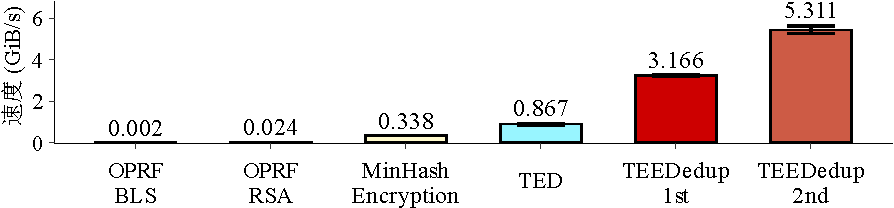
\includegraphics[width=\linewidth]{../pic/sgxdedup/plot/exp_a2/expa2_keyGenPerformance.pdf}
        \caption{单客户端密钥生成性能对比}
    \end{figure}

    \begin{itemize}
        \item TEEDedup提出的密钥生成方案相比OPRF-BLS和OPRF-RSA在第一轮(不含推测性加密)中实现了1,583倍和131.9倍的性能提升,而第二轮基于推测性加密,TEEDedup将第一轮的密钥生成速度再次提高了67.8\%
    \end{itemize}
\end{frame}

\begin{frame}{会话密钥更新开销}
    \begin{figure}[!htb]
        \centering
        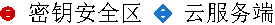
\includegraphics[height=11pt]{../pic/sgxdedup/plot/exp_a5/expa5_keyRegression_time_legend.pdf}
        \begin{tabular}{@{\ }c@{\ }c}
            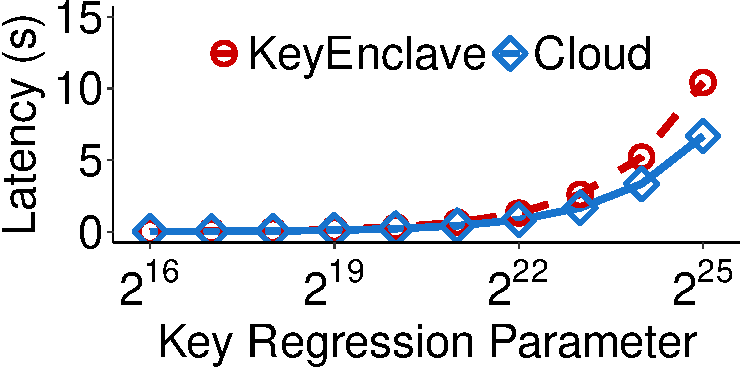
\includegraphics[width=0.49\textwidth]{../pic/sgxdedup/plot/exp_a5/expa5_keyRegression_time.pdf} &
            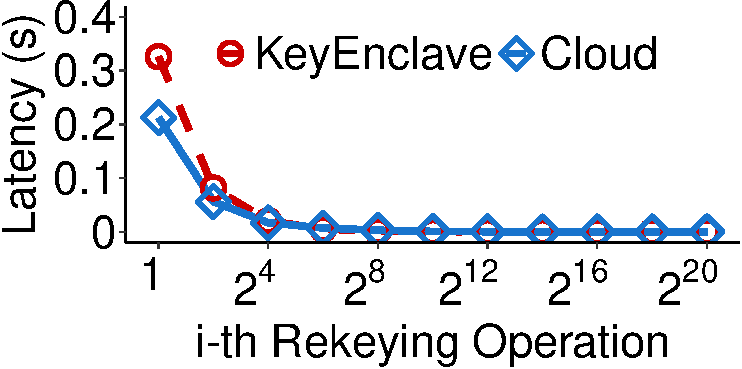
\includegraphics[width=0.49\textwidth]{../pic/sgxdedup/plot/exp_a5/expa5_keyRegression_time_default.pdf} \\
            \mbox{\small (a)密钥回归参数的影响}                                                              &
            \mbox{\small (b)密钥回归执行次数的影响}
        \end{tabular}
        \caption{会话密钥更新延迟}
        \label{fig:sgxdedup-rekeyingLatency}
    \end{figure}
    \begin{itemize}
        \item 密钥更新开销较低:密钥安全区的密钥更新延迟为0.040\,s,云服务端约为0.027\,s。
        \item 安全区处理密集计算的能力较弱,其密钥更新延迟相较云服务端高1.22~1.56倍。
    \end{itemize}
\end{frame}

\begin{frame}{数据块所有权证明效率}
    \begin{figure}[!htb]
        \begin{minipage}[t]{0.47\textwidth}
            \centering
            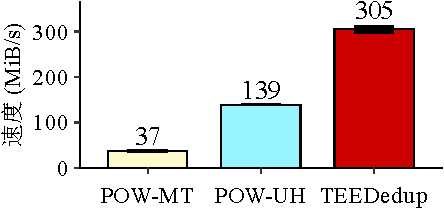
\includegraphics[width=\linewidth]{../pic/sgxdedup/plot/exp_a4/expa4_powPerformance.pdf}
            \caption{数据所有权证明的计算性能(不含网络开销)}
            \label{fig:sgxdedup-pow-comparison}
        \end{minipage}%
        \hspace{0.2in}
        \begin{minipage}[t]{0.47\textwidth}
            \centering
            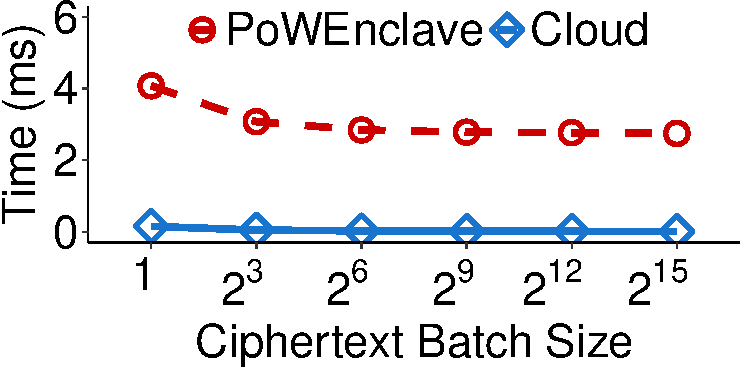
\includegraphics[width=\linewidth]{../pic/sgxdedup/plot/exp_a4/expa4_powBatchSize_breakdown.pdf}
            \caption{所有权证明的计算开销vs.批量大小(单位:ms/MiB)}
            \label{fig:sgxdedup-multiClientThroughput}
        \end{minipage}%
    \end{figure}
    \begin{itemize}
        \item 由于\sysnameS 避免了客户端中的纠删码编码和Merkle树构造,实现了相较于PoW-MT 8.2倍的性能提升。相较于安全性较弱的PoW-UH实现了2.2倍的性能提升。
        \item 云服务端的计算时间开销很低(低于0.05\,ms),而所有权证明安全区的计算时间随着批量大小增大从4.1\,ms减少到 2.7\,ms。
    \end{itemize}
\end{frame}

\begin{frame}{\sysnameS 原型系统性能}
    \begin{figure}[!htb]
        \centering
        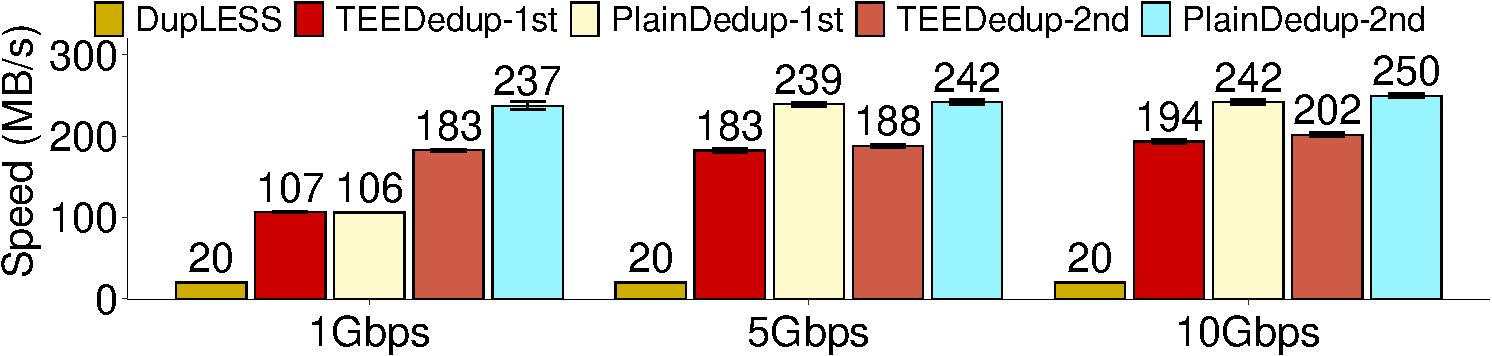
\includegraphics[width=0.646\textwidth]{../pic/sgxdedup/plot/exp_b1/upload_network_speed_bar.pdf}
        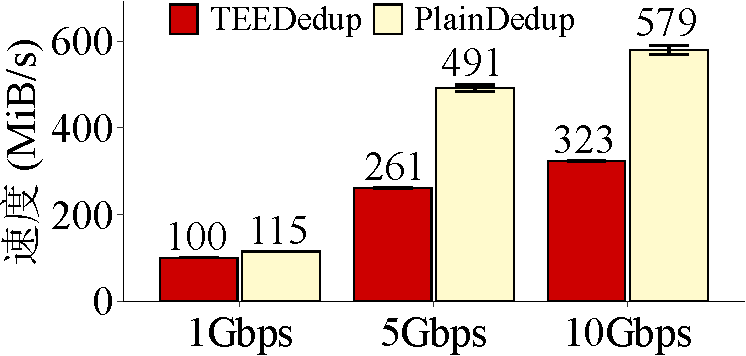
\includegraphics[width=0.324\textwidth]{../pic/sgxdedup/plot/exp_b1/download_network_speed_bar.pdf}
        \\
        \hspace{1.1in} {\small (a) 上传} \hspace{1.4in}
        {\small (b) 下载}\\
        \caption{单客户端在不同网络速度下的上传/下载性能}
        \label{fig:sgxdedup-singleClientThroughput}
    \end{figure}

    \begin{itemize}
        \item \sysnameS 在第一轮和第二轮上传中分别相对DupLESS实现了8.1倍和9.6倍的性能提升。
        \item 与不安全的PlainDedup相比,\sysnameS 仅导致两轮上传速度分别下降约17.5\%和21.4\%。
    \end{itemize}
\end{frame}

\subsection{\sysnameF 检测方案}

\begin{frame}{密文数据块的相似性检测}
    \begin{columns}
        \begin{column}{.5\textwidth}
            \vspace{-1em}
            \begin{figure}[!htb]
                \centering
                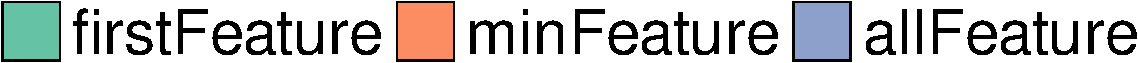
\includegraphics[width=0.8\linewidth]{../pic/featurespy/plot/detection/syn/synBarPlotDetect_legend.pdf}\\
                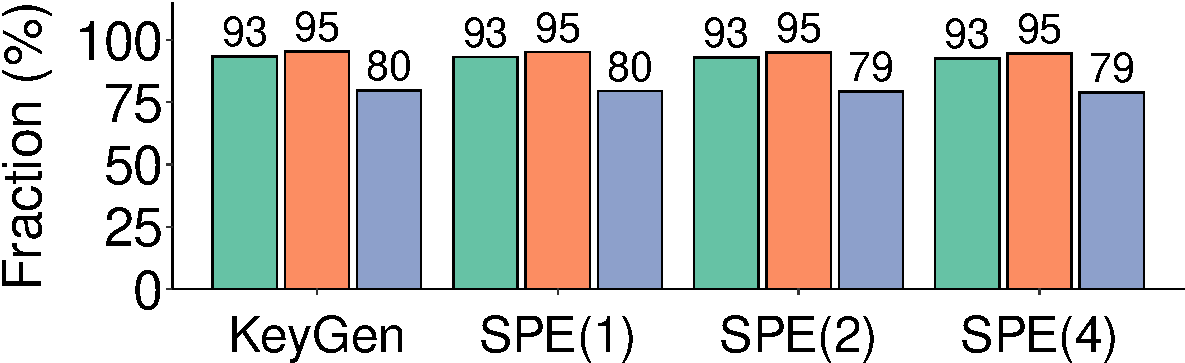
\includegraphics[width=\linewidth]{../pic/featurespy/plot/detection/syn/syn-p1-q4-detect.pdf}  \\
                \vspace{-3pt}
                \mbox{\fontsize{8.0pt}{\baselineskip}\selectfont (a) $\textrm{SYNChunk}(1, 4)$}                                                        \\
                \vspace{-3pt}
                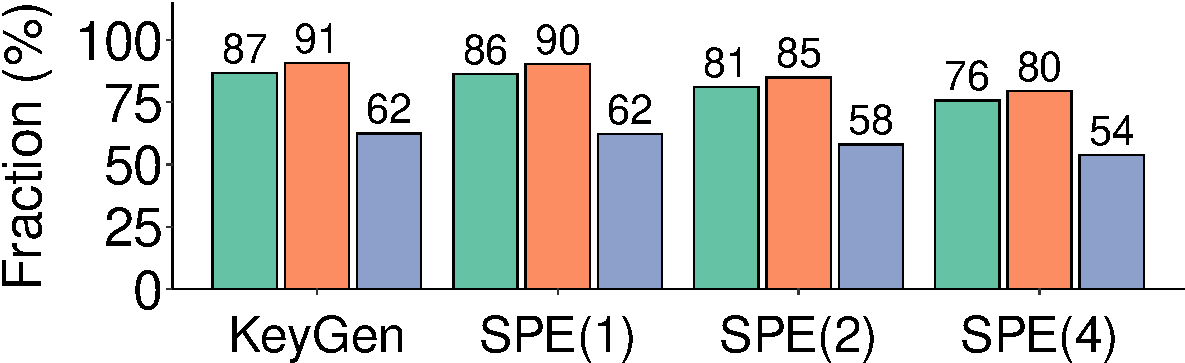
\includegraphics[width=\linewidth]{../pic/featurespy/plot/detection/syn/syn-p2-q8-detect.pdf}    \\
                \vspace{-3pt}
                \mbox{\fontsize{8.0pt}{\baselineskip}\selectfont (b) $\textrm{SYNChunk}(2, 8)$}                                                          \\
                \vspace{-3pt}
                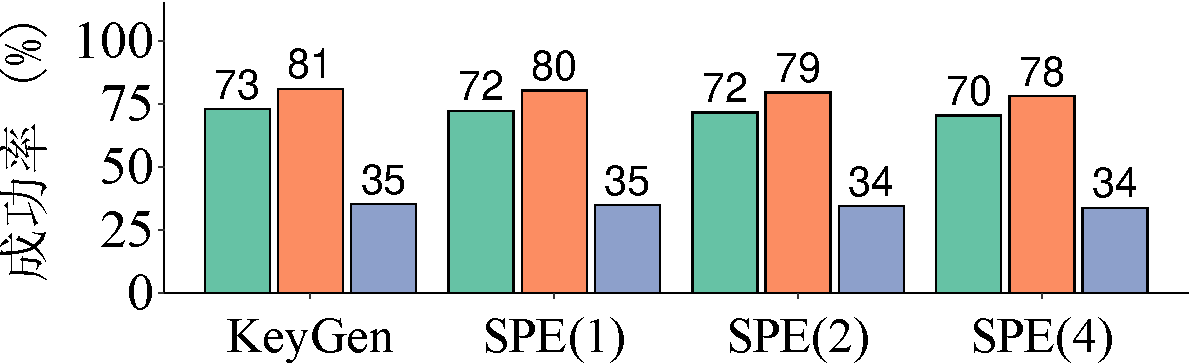
\includegraphics[width=\linewidth]{../pic/featurespy/plot/detection/syn/syn-p4-q16-detect.pdf} \\
                \vspace{-3pt}
                \mbox{\fontsize{8.0pt}{\baselineskip}\selectfont (c) $\textrm{SYNChunk}(4, 16)$}                                                       \\
                \vspace{-3pt}
                \caption{密文数据块的相似性检测效果}
                \label{fig:featurespy-expDetectionSynDetect}
            \end{figure}
        \end{column}
        \begin{column}{.5\textwidth}
            \begin{itemize}
                \item {\tt minFeature}方案对数据块内容的随机变化更不敏感。
                \item 相似性保留加密在加密后保留了较高的相似性: 通过检查密文数据块中的相似性指标,在SYNChunk$(1,4)$、SYNChunk$(2,8)$、SYNChunk$(4,16)$数据集中分别检测到至多95.2\%、90.4\%、80.2\%的相似数据块。
            \end{itemize}
        \end{column}
    \end{columns}
\end{frame}

\begin{frame}{推测内容攻击检测效果案例分析}
    \begin{columns}
        \begin{column}{.6\textwidth}
            \vspace{-1em}
            \begin{figure}[!htb]
                \centering
                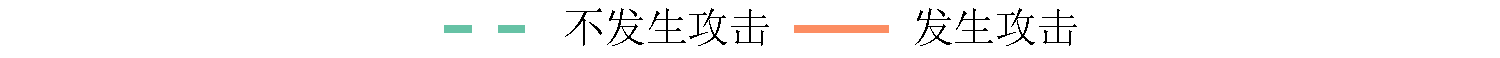
\includegraphics[width=\linewidth]{../pic/featurespy/plot/detection/overall/prefixDistribution_legend.pdf}\\
                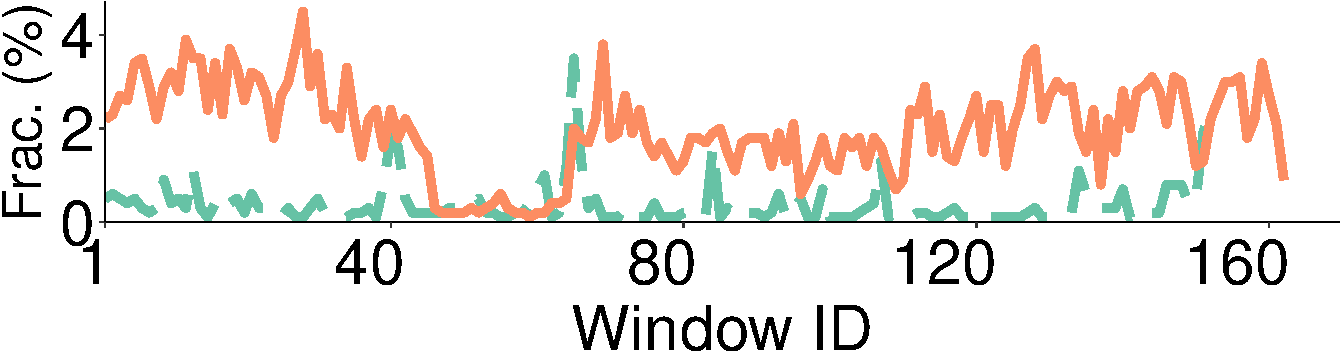
\includegraphics[width=\linewidth]{../pic/featurespy/plot/detection/overall/prefixDistribution-1000-Linux-min.pdf}\\
                \caption{Linux最新快照在包含/不包含攻击行为时每个窗口(W=1\,K)的相似性指标的频率特征。}
                \label{fig:featurespy-expDetectionOverall}
            \end{figure}
            \vspace{-2em}
            \begin{figure}[!htb]
                \centering
                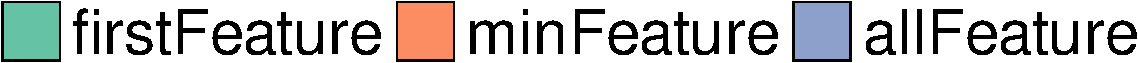
\includegraphics[width=0.66\linewidth]{../pic/featurespy/plot/detection/overall/effectiveness-falsePositive_legend.pdf}
                \vspace{5pt}\\
                \begin{tabular}{@{\ }c@{\ }c}
                    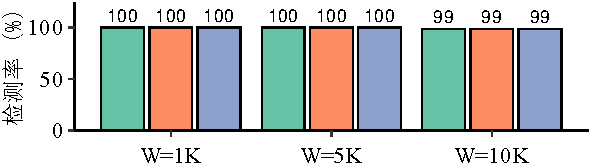
\includegraphics[width=0.66\linewidth]{../pic/featurespy/plot/detection/overall/effectivenessLinux.pdf} &
                    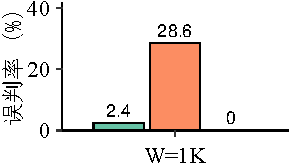
\includegraphics[width=0.33\linewidth]{../pic/featurespy/plot/detection/overall/falsePositiveLinux.pdf}   \\
                    \mbox{\small (a) 检测率}                                                                                &
                    \mbox{\small (b) 误判率}                                                                                  \\
                \end{tabular}
                \caption{Linux数据集中总体检测率和误判率}
                \label{fig:featurespy-expDetectionOverallFalsePositive}
            \end{figure}
        \end{column}
        \begin{column}{.4\textwidth}
            \begin{itemize}
                \item 在对所有窗口大小使用相同检测阈值T时,随窗口大小增大误报率降低(W=5,10\,K时为0)。
                \item {\tt minFeature}方案检测到更多相似数据块,相较于其他两种方案产生更高误报率。
            \end{itemize}
        \end{column}
    \end{columns}
\end{frame}

\subsection{\prototype 原型系统}

\begin{frame}{\prototype 原型系统性能}
    \begin{figure}[!htb]
        \centering
        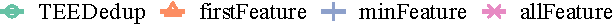
\includegraphics[width=0.7\textwidth]{../pic/featurespy/plot/performance/multiClient/legend.pdf}
        \vspace{5pt}\\
        \begin{tabular}{@{\ }c@{\ }c@{\ }c}
            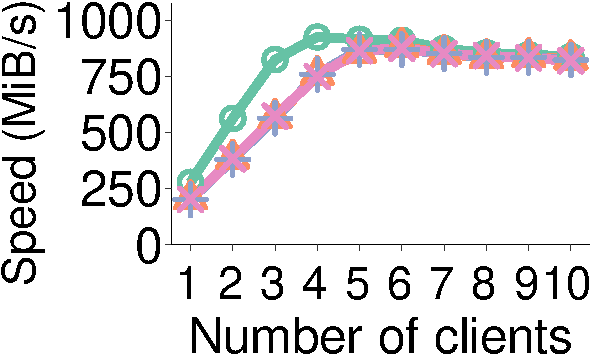
\includegraphics[width=0.32\textwidth]{../pic/featurespy/plot/performance/multiClient/upload_1st_line.pdf} &
            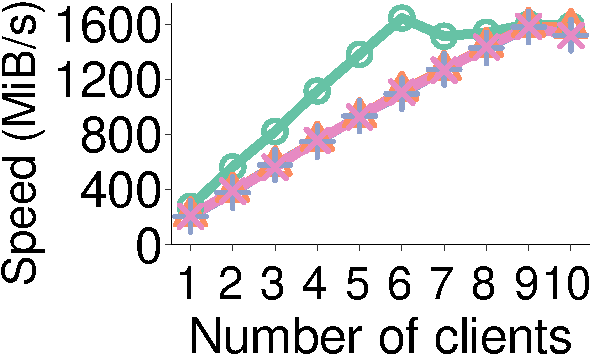
\includegraphics[width=0.32\textwidth]{../pic/featurespy/plot/performance/multiClient/upload_2nd_line.pdf} &
            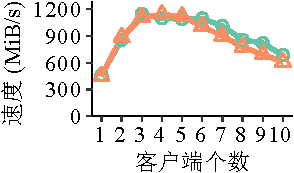
\includegraphics[width=0.32\textwidth]{../pic/featurespy/plot/performance/multiClient/download_line.pdf}     \\
            {\small (a)第一轮上传}                                                                                     &
            {\small (b)第二轮上传}                                                                                     &
            {\small (c)下载}
        \end{tabular}
        \caption{多客户端上传/下载性能。所有\prototype 实例的下载速度均相同的,本文将它们(橙色)与 \sysnameS(绿色)进行比较。}
        \label{fig:featurespy-expMultiClientThroughput}
    \end{figure}

    \begin{itemize}
        \item \sysnameS (4客户端聚合上传速度924.9\,MiB/s)比\prototype 更早达到峰值性能(6客户端聚合上传速度882.2\,MiB/s)
    \end{itemize}
\end{frame}

\subsection{\prototype 实际工作负载测试}

\begin{frame}{实际工作负载网络资源开销}
    \begin{figure}[!htb]
        \centering
        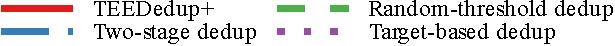
\includegraphics[height=16pt]{../pic/featurespy/plot/bandwidth/upload_traffic_legend.pdf}
        \vspace{5pt} \\
        \begin{tabular}{@{\ }c@{\ }c@{\ }c@{\ }c}
            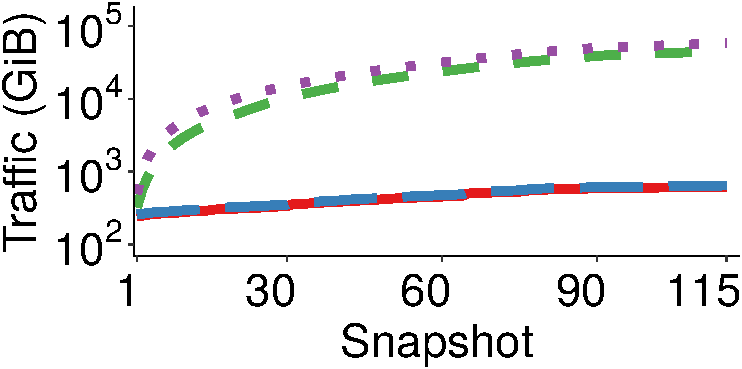
\includegraphics[width=0.45\linewidth]{../pic/featurespy/plot/bandwidth/upload_traffic_fsl.pdf} &
            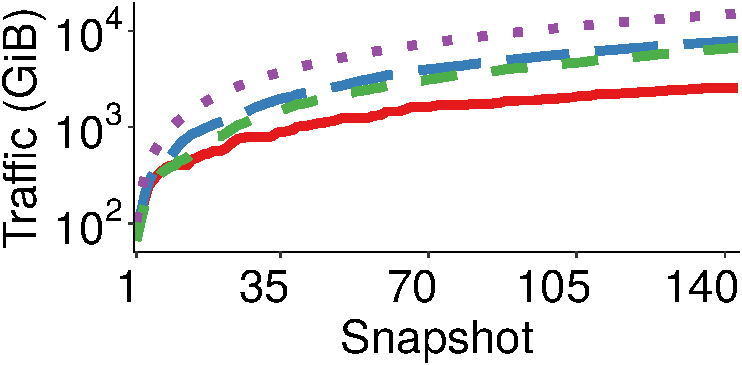
\includegraphics[width=0.45\linewidth]{../pic/featurespy/plot/bandwidth/upload_traffic_ms.pdf}                          \\
            {\small (a) FSL数据集}                                                                          & {\small (b) MS数据集}
        \end{tabular}
        \caption{上传每个快照后累积的网络流量。}
        \label{fig:featurespy-expNetworkTraffic}
    \end{figure}

    \begin{itemize}
        \item \prototype 相较于目标端重复数据删除的网络流量在FSL数据集中减少了98.9\%,并在MS数据集中减少了83.1\%。
    \end{itemize}
\end{frame}

\begin{frame}{实际工作负载性能分析}
    \begin{figure}[!htb]
        \centering
        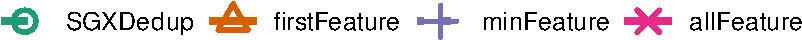
\includegraphics[height=8pt]{../pic/featurespy/plot/performance/LANTrace/trace_legend_upload.pdf}\\
        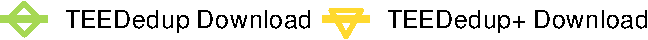
\includegraphics[height=8pt]{../pic/featurespy/plot/performance/LANTrace/trace_legend_download.pdf}
        \vspace{5pt} \\
        \begin{tabular}{@{\ }c@{\ }c}
            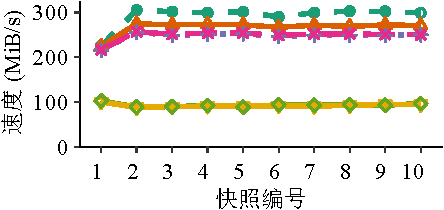
\includegraphics[width=0.45\linewidth]{../pic/featurespy/plot/performance/LANTrace/trace_fsl.pdf} &
            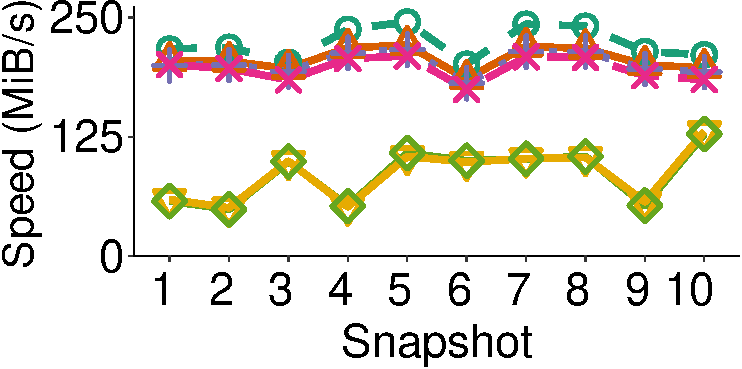
\includegraphics[width=0.45\linewidth]{../pic/featurespy/plot/performance/LANTrace/trace_ms.pdf}    \\
            \mbox{\small (a) FSL}                                                                             &
            \mbox{\small (b)  MS}                                                                               \\
        \end{tabular}
        \caption{实际工作负载下上传/下载性能}
        \label{fig:featurespy-traceDrivenThroughput}
    \end{figure}

    \begin{itemize}
        \item 与\sysnameS 相比,\prototype 的{\tt firstFeature}、{\tt minFeature}和{\tt allFeature}实例的上传性能分别降低8.8\%、15.7\%和15.0\%,下载性能降低了0.8\%。
    \end{itemize}
\end{frame}

\section{个人成果}

\begin{frame}[allowframebreaks]{攻读硕士学位期间取得的成果}
    \newcommand{\bstlabelmark}{lo}
    \nocite{*}
    \bibliographystyle{thesis-uestc}
    \bibliography{publication}
\end{frame}

\begin{frame}
    \begin{center}
        {\Huge 衷心感谢老师倾听}

        {\Huge 请各位老师指正!}
    \end{center}
\end{frame}

\end{document}